%% bare_jrnl.tex
%% V1.4b
%% 2015/08/26
%% by Michael Shell
%% see http://www.michaelshell.org/

\documentclass[twoside,journal]{IEEEtran}

\usepackage{mycommands}

\begin{document}



\title{Gofem User Manual}

\author{Dorival~M.~Pedroso%
\thanks{School of Civil Engineering, The University of Queensland, St Lucia QLD 4072, Australia,
e-mail:d.pedroso@uq.edu.au}}

\markboth{User Manual}
{Gofem}

\maketitle




\begin{abstract}

Gofem is a framework to implement solutions of partial differential equations using the finite
element method. Focus is given to the equations derived from the theory of porous media in addition
to some structural mechanics problems.

\end{abstract}

\begin{IEEEkeywords}
partial differential equations, finite element method, parallel computing, porous media mechanics
\end{IEEEkeywords}



\section{Introduction}
\label{sec:intro}

Gofem (Go Finite Element Method) is an implementation of the finite element method (FEM) in Go
language for applications in solid mechanics. The code aims to be as general as possible and has a
focus on porous media mechanics. Nonetheless, classical plasticity and the solution of multi-physics
coupled problems are also targeted by Gofem. Efficiency is a goal as long as the quality of code and
code maintenance is not penalised. The computational efficiency is achieved by parallel computing
using message passage interface (MPI). Several unit tests are employed for every detail of the code
and its usage aims to be comprehensive. Gofem depends on the Go Scientific Library (Gosl) and was
developed for obtaining the results presented in a number of journal papers, including
\cite{pedroso:15a} and \cite{pedroso:15b}.


\section{Linearised problem and Solution structure}

The solution structure is defined by a collection of all degrees of freedom of all nodes in the
mesh. This is indicated by $\vC{y}$.

\begin{equation}
    \vC{y} = \begin{Bmatrix}
        u_x^0 \\ u_y^1 \\ \ldots \\ p_\ell^0 \\ p_g^0 \\ \ldots
    \end{Bmatrix}
\end{equation}


\section{Finite element method}

This section presents a quick introduction to the finite element method (FEM) as considered in
Gofem.

\subsection{Overview of main structures}


\begin{figure} \centering
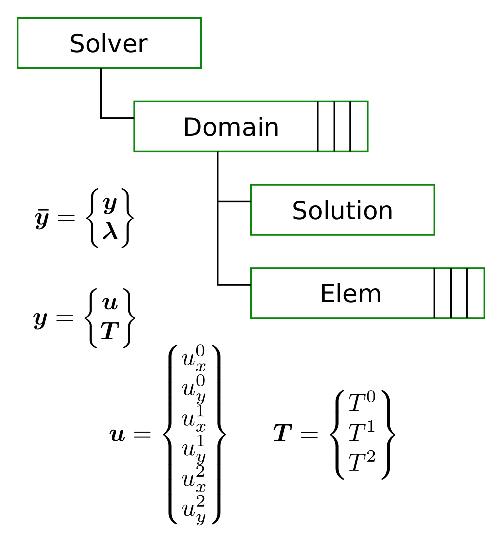
\includegraphics[scale=0.7]{./figs/overview.eps}
\caption{Overview}
\label{fig:overview}
\end{figure}


\subsection{Pinned frames: Linear elastic rod element}

The element equations are:
\begin{equation}
\vr_u = \tSe{K} \, \vu - \vf
\end{equation}




\subsection{Diffusion equation}



\section{Conclusion}
\label{sec:conclusion}

Gofem is a powerful framework to implement FEM solutions. It is also versatile and easy to be
extended.



\section*{Acknowledgment}

The support from The University of Queensland, Australia and the Australian Research Council are
gratefully acknowledged.



\bibliographystyle{IEEEtran}
\bibliography{mydatabase}

\end{document}
